%!TEX encoding = UTF-8 Unicode
\documentclass[french, a4paper, 12pt]{article}



%% Langue et compilation

\usepackage[utf8]{inputenc}
\usepackage[T1]{fontenc}
\usepackage[french]{babel}

%% LISTE DES PACKAGES

\usepackage{mathtools}     % package de base pour les maths
\usepackage{amsmath}       % mathematical type-setting
\usepackage{amssymb}       % symbols speciaux pour les maths
\usepackage{textcomp}      % symboles speciaux pour el text
\usepackage{gensymb}       % commandes generiques \degree etc...
\usepackage{tikz}          % package graphique
\usepackage{wrapfig}       % pour entourer a cote d'une figure
\usepackage{color}         % package des couleurs
\usepackage{xcolor}        % autre package pour les couleurs
\usepackage{pgfplots}      % pacakge pour creer des graph
\usepackage{epsfig}        % permet d'inclure des graph en .eps
\usepackage{graphicx}      % arguments dans includegraphics
\usepackage{pdfpages}      % permet d'insérer des pages pdf dans le document
\usepackage{subfig}        % permet de creer des sous-figure
\usepackage{pst-all}       % utile pour certaines figures en pstricks
\usepackage{lipsum}        % package qui permet de faire des essais
\usepackage{array}         % permet de faire des tableaux
\usepackage{multicol}      % plusieurs colonnes sur une page
\usepackage{enumitem}      % pro­vides user con­trol: enumerate, itemize and description
\usepackage{hyperref}      % permet de creer des hyperliens dans le document
\usepackage{lscape}        % permet de mettre une page en mode paysage
\usepackage{lmodern}       % permet d'avoir certains "fonts" de bonen qualite
\usepackage{fancyhdr}      % Permet de mettre des informations en hau et en bas de page      
\usepackage[framemethod=tikz]{mdframed} % breakable frames and coloured boxes
\usepackage[top=1.5cm, bottom=1.5cm, left=2.5cm, right=2.5cm]{geometry} % donne les marges
\usepackage[font=normalsize, labelfont=bf,labelsep=endash, figurename=Fig.]{caption} % permet de changer les legendes des figures
\usepackage{lewis}
\usepackage{bohr}
\usepackage{chemfig}
\usepackage{chemist}

%% LIBRAIRIES

\usetikzlibrary{plotmarks} % librairie pour les graphes
\usetikzlibrary{patterns}  % necessaire pour certaines choses predefinies sur tikz
\usetikzlibrary{shadows}   % ombres des encadres
\usetikzlibrary{backgrounds} % arriere plan des encadres


%% MISE EN PAGE

\pagestyle{fancy}     % Défini le style de la page

\renewcommand{\headrulewidth}{1pt}      % largeur du trait en haut de la page
\fancyhead[L]{Seconde générale}         % info coin haut gauche
\fancyhead[R]{Lycée Jean Guéhenno}  % info coin haut droit

% bas de la page
\renewcommand{\footrulewidth}{1pt}      % largeur du trait en bas de la page
\fancyfoot[L]{G. \bsc{LE DOUDIC}}  % info coin bas gauche
\fancyfoot[R]{TP 4 : Famille chimique}                         % info coin bas droit


\setlength{\columnseprule}{1pt} 
\setlength{\columnsep}{30pt}



%% NOUVELLES COMMANDES 

\DeclareMathOperator{\e}{e} % permet d'ecrire l'exponentielle usuellement


\newcommand{\gap}{\vspace{0.15cm}}   % defini une commande pour sauter des lignes
\renewcommand{\vec}{\overrightarrow} % permet d'avoir une fleche qui recouvre tout le vecteur
\newcommand{\bi}{\begin{itemize}}    % begin itemize
\newcommand{\ei}{\end{itemize}}      % end itemize
\newcommand{\bc}{\begin{center}}     % begin center
\newcommand{\ec}{\end{center}}       % end center
\newcommand\opacity{1}               % opacity 
\pgfsetfillopacity{\opacity}

\newcommand*\Laplace{\mathop{}\!\mathbin\bigtriangleup} % symbole de Laplace

\frenchbsetup{StandardItemLabels=true} % je ne sais plus

\newcommand{\smallO}[1]{\ensuremath{\mathop{}\mathopen{}o\mathopen{}\left(#1\right)}} % petit o

\newcommand{\cit}{\color{blue}\cite} % permet d'avoir les citations de couleur bleues
\newcommand{\bib}{\color{black}\bibitem} % paragraphe biblio en noir et blanc
\newcommand{\bthebiblio}{\color{black} \begin{thebibliography}} % idem necessaire sinon bug a cause de la couleur
\newcommand{\ethebiblio}{\color{black} \end{thebibliography}}   % idem
%%% TIKZ


%% COULEURS 


\definecolor{definitionf}{RGB}{220,252,220}
\definecolor{definitionl}{RGB}{39,123,69}
\definecolor{definitiono}{RGB}{72,148,101}

\definecolor{propositionf}{RGB}{255,216,218}
\definecolor{propositionl}{RGB}{38,38,38}
\definecolor{propositiono}{RGB}{109,109,109}

\definecolor{theof}{RGB}{255,216,218}
\definecolor{theol}{RGB}{160,0,4}
\definecolor{theoo}{RGB}{221,65,100}

\definecolor{avertl}{RGB}{163,92,0}
\definecolor{averto}{RGB}{255,144,0}

\definecolor{histf}{RGB}{241,238,193}

\definecolor{metf}{RGB}{220,230,240}
\definecolor{metl}{RGB}{56,110,165}
\definecolor{meto}{RGB}{109,109,109}


\definecolor{remf}{RGB}{230,240,250}
\definecolor{remo}{RGB}{150,150,150}

\definecolor{exef}{RGB}{240,240,240}

\definecolor{protf}{RGB}{247,228,255}
\definecolor{protl}{RGB}{105,0,203}
\definecolor{proto}{RGB}{174,88,255}

\definecolor{grid}{RGB}{180,180,180}

\definecolor{titref}{RGB}{230,230,230}

\definecolor{vert}{RGB}{23,200,23}

\definecolor{violet}{RGB}{180,0,200}

\definecolor{copper}{RGB}{217, 144, 88}

%% Couleur des ref

\hypersetup{
	colorlinks=true,
	linkcolor=black,
	citecolor=blue,
	urlcolor=black
		   }

%% CADRES


% %%%%%%%%%% DEFINITION
% \newmdenv[tikzsetting={fill=definitionf}, linewidth=2pt, linecolor=definitionl, outerlinewidth=0pt, innertopmargin=5pt, innerbottommargin=5pt, innerleftmargin=5pt, innerrightmargin=5pt, leftmargin=0pt]{definition}

% \newmdenv[ tikzsetting={drop shadow={ shadow xshift=1ex, shadow yshift=-0.5em, fill=definitiono, opacity=1, every shadow } }, outerlinewidth=2pt, outerlinecolor=white, linecolor=white, innertopmargin=0pt, innerbottommargin=0pt, innerleftmargin=0pt, innerrightmargin=0pt]{ombredef}


% %%%%%%%%%% THEOREME

% \newmdenv[tikzsetting={fill=theof}, linewidth=2pt, linecolor=theol, outerlinewidth=0pt, innertopmargin=5pt, innerbottommargin=5pt, innerleftmargin=5pt, innerrightmargin=5pt, leftmargin=0pt]{theo}

% \newmdenv[ tikzsetting={drop shadow={ shadow xshift=1ex, shadow yshift=-0.5em, fill=theoo, opacity=1, every shadow } }, outerlinewidth=2pt, outerlinecolor=white, linecolor=white, innertopmargin=0pt, innerbottommargin=0pt, innerleftmargin=0pt, innerrightmargin=0pt]{ombretheo}


% %%%%%%%%%% METHODE

% \newmdenv[tikzsetting={fill=metf}, linewidth=2pt, linecolor=metl, outerlinewidth=0pt, innertopmargin=5pt, innerbottommargin=5pt, innerleftmargin=5pt, innerrightmargin=5pt, leftmargin=0pt]{met}

% \newmdenv[ tikzsetting={drop shadow={ shadow xshift=1ex, shadow yshift=-0.5em, fill=meto, opacity=1, every shadow } }, outerlinewidth=2pt, outerlinecolor=white, linecolor=white, innertopmargin=0pt, innerbottommargin=0pt, innerleftmargin=0pt, innerrightmargin=0pt]{ombremet}



%%%%%%%%%%% RQ

\newmdenv[tikzsetting={fill=remf}, linewidth=2pt, linecolor=remf, outerlinewidth=0pt, innertopmargin=5pt, innerbottommargin=5pt, innerleftmargin=5pt, innerrightmargin=5pt, leftmargin=0pt]{remarque}

\newmdenv[ tikzsetting={drop shadow={ shadow xshift=1ex, shadow yshift=-0.5em, fill=remo, opacity=1, every shadow } }, outerlinewidth=2pt, outerlinecolor=white, linecolor=white, innertopmargin=0pt, innerbottommargin=0pt, innerleftmargin=0pt, innerrightmargin=0pt]{ombreremarque}

%%%%%%%%%%% Cadre pour le titre

\tikzset{every shadow/.style={opacity=1}}

\global\mdfdefinestyle{doc}{backgroundcolor=white, shadow=true, shadowcolor=propositiono, linewidth=1pt, linecolor=black, shadowsize=5pt}
\global\mdfdefinestyle{titr}{backgroundcolor=metf, shadow=true, shadowcolor=propositiono, linewidth=1pt, linecolor=black, shadowsize=5pt}
\global\mdfdefinestyle{theo}{backgroundcolor=theof, shadow=true, shadowcolor=theoo, linewidth=1pt, linecolor=theol, shadowsize=5pt}
\global\mdfdefinestyle{prop}{backgroundcolor=theof, shadow=true, shadowcolor=propositiono, linewidth=1pt, linecolor=theol, shadowsize=5pt}
\global\mdfdefinestyle{def}{backgroundcolor=definitionf, shadow=true, shadowcolor=definitiono, linewidth=1pt, linecolor=definitionl, shadowsize=5pt}
\global\mdfdefinestyle{histo}{backgroundcolor=histf, shadow=true, shadowcolor=propositiono, linewidth=1pt, linecolor=black, shadowsize=5pt}
\global\mdfdefinestyle{avert}{backgroundcolor=white, shadow=true, shadowcolor=averto, linewidth=1pt, linecolor=avertl, shadowsize=5pt}
\global\mdfdefinestyle{met}{backgroundcolor=metf, shadow=true, shadowcolor=meto, linewidth=1pt, linecolor=metl, shadowsize=5pt}
\global\mdfdefinestyle{rem}{backgroundcolor=metf, shadow=true, shadowcolor=meto, linewidth=1pt, linecolor=metf, shadowsize=5pt}
\global\mdfdefinestyle{exo}{backgroundcolor=exef, shadow=true, shadowcolor=propositiono, linewidth=1pt, linecolor=exef, shadowsize=5pt}
\global\mdfdefinestyle{not}{backgroundcolor=definitionf, shadow=true, shadowcolor=propositiono, linewidth=1pt, linecolor=black, shadowsize=5pt}
\global\mdfdefinestyle{proto}{backgroundcolor=protf, shadow=true, shadowcolor=proto, linewidth=1pt, linecolor=protl, shadowsize=5pt}

%%%%%%
\definecolor{cobalt}{rgb}{0.0, 0.28, 0.67}
\definecolor{applegreen}{rgb}{0.55, 0.71, 0.0}

\usepackage{tcolorbox}
  \tcbuselibrary{most}
  \tcbset{colback=cobalt!5!white,colframe=cobalt!75!black}



\newtcolorbox{definition}[1]{
	colback=applegreen!5!white,
  	colframe=applegreen!65!black,
	fonttitle=\bfseries,
  	title={#1}}
\newtcolorbox{Programme}[1]{
	colback=cobalt!5!white,
  	colframe=cobalt!65!black,
	fonttitle=\bfseries,
  	title={#1}}  

\newtcolorbox{Exercice}[1]{
  colback=cobalt!5!white,
  colframe=cobalt!65!black,
  fonttitle=\bfseries,
  title={#1}}  

  \newtcolorbox{Protocol}[1]{
  colback=cyan!5!white,
  colframe=cyan!65!black,
  fonttitle=\bfseries,
  title={#1}}  

\newtcolorbox{Resultat}[1]{
	colback=theof,%!5!white,
	colframe=theoo!85!black,
  fonttitle=\bfseries,
	title={#1}} 	


\def\width{12}
\def\hauteur{5}

\setlength{\parskip}{0pt}%
\setlength{\parindent}{18pt}


%% MODIFICATION DE CHAPTER  
\makeatletter
\def\@makechapterhead#1{%
  %%%%\vspace*{50\p@}% %%% removed!
  {\parindent \z@ \raggedright \normalfont
    \ifnum \c@secnumdepth >\m@ne
        \huge\bfseries \@chapapp\space \thechapter
        \par\nobreak
        \vskip 20\p@
    \fi
    \interlinepenalty\@M
    \Huge \bfseries #1\par\nobreak
    \vskip 40\p@
  }}
\def\@makeschapterhead#1{%
  %%%%%\vspace*{50\p@}% %%% removed!
  {\parindent \z@ \raggedright
    \normalfont
    \interlinepenalty\@M
    \Huge \bfseries  #1\par\nobreak
    \vskip 40\p@
  }}
  
  \newcommand{\isotope}[3]{%
     \settowidth\@tempdimb{\ensuremath{\scriptstyle#1}}%
     \settowidth\@tempdimc{\ensuremath{\scriptstyle#2}}%
     \ifnum\@tempdimb>\@tempdimc%
         \setlength{\@tempdima}{\@tempdimb}%
     \else%
         \setlength{\@tempdima}{\@tempdimc}%
     \fi%
    \begingroup%
    \ensuremath{^{\makebox[\@tempdima][r]{\ensuremath{\scriptstyle#1}}}_{\makebox[\@tempdima][r]{\ensuremath{\scriptstyle#2}}}\text{#3}}%
    \endgroup%
  }%

\makeatother

\usepackage{lewis}
\usepackage{bohr}
\usepackage{chemfig}
\usepackage{chemist}
\usepackage{tabularx}
\usepackage{pgf-spectra}

\tikzset{
  % style to apply some styles to each segment of a path
  on each segment/.style={
    decorate,
    decoration={
      show path construction,
      moveto code={},
      lineto code={
        \path [#1]
        (\tikzinputsegmentfirst) -- (\tikzinputsegmentlast);
      },
      curveto code={
        \path [#1] (\tikzinputsegmentfirst)
        .. controls
        (\tikzinputsegmentsupporta) and (\tikzinputsegmentsupportb)
        ..
        (\tikzinputsegmentlast);
      },
      closepath code={
        \path [#1]
        (\tikzinputsegmentfirst) -- (\tikzinputsegmentlast);
      },
    },
  },
  % style to add an arrow in the middle of a path
  mid arrow/.style={postaction={decorate,decoration={
        markings,
        mark=at position .5 with {\arrow[#1]{stealth}}
      }}},
}


\usepackage{tikz}
\usetikzlibrary{3d, shapes.multipart}

% Styles
\tikzset{>=latex} % for LaTeX arrow head
\tikzset{axis/.style={black, thick,->}}
\tikzset{vector/.style={>=stealth,->}}
\tikzset{every text node part/.style={align=center}}
\usepackage{amsmath} % for \text
 
\usetikzlibrary{decorations.pathreplacing,decorations.markings}
% %%% TEST EXERCIES SOLUTIONS
% \usepackage{answers}
% %\usepackage[nosolutionfiles]{answers}
% % def d'un environnement Exercise numerote
% \newtheorem{Exc}{Exercise}
% \newenvironment{Ex}{\begin{Exc}\normalfont}%
%                    {\end{Exc}}
% % Trois types de solutions sont proposes
% \Newassociation{solution}{Soln}{test}
% \Newassociation{hint}{Hint}{test}
% \Newassociation{Solution}{sSol}{testtwo}
% \newcommand{\prehint}{~[Hint]}
% \newcommand{\presolution}{~[Solution]}
% \newcommand{\preSolution}{~[Homework]}
% % test
% \newcommand{\Opentesthook}[2]%
%    {\Writetofile{#1}%
%     {\protect\section{#1: #2}}}
% % introduction de la solution
% \renewcommand{\Solnlabel}[1]{\emph{Solution #1}}
% \renewcommand{\Hintlabel}[1]{\emph{Hint #1}}
% \renewcommand{\sSollabel}[1]{\emph{Solution to #1}}


%%
%%
%% DEBUT DU DOCUMENT
%%
\setlength{\tabcolsep}{7pt}

\renewcommand{\arraystretch}{2}


%% COMMANDE Exercice

\newcommand{\exo}[3]{
	\begin{mdframed}[style=exo, leftmargin=0pt, rightmargin=0pt, innertopmargin=8pt, innerbottommargin=8pt, innerrightmargin=10pt, innerleftmargin=10pt]

		\noindent \textbf{Exercice #1 - #2}\medskip

		#3
	\end{mdframed}
}

\newcommand{\doc}[3]{
	\begin{mdframed}[style=doc, leftmargin=0pt, rightmargin=0pt, innertopmargin=8pt, innerbottommargin=8pt, innerrightmargin=10pt, innerleftmargin=10pt]

		\noindent \textbf{Document #1 - #2}\medskip

		#3
	\end{mdframed}
}

\newcommand{\defi}[3]{
	\begin{mdframed}[style=def, leftmargin=0pt, rightmargin=0pt, innertopmargin=8pt, innerbottommargin=8pt, innerrightmargin=10pt, innerleftmargin=10pt]

		\noindent \textbf{Document #1 - #2}\medskip

		#3
	\end{mdframed}
}

\begin{document}


%%%%%%
\tikzset{every shadow/.style={opacity=1}}

\global\mdfdefinestyle{doc}{backgroundcolor=white, shadow=true, shadowcolor=propositiono, linewidth=1pt, linecolor=black, shadowsize=5pt}
\global\mdfdefinestyle{titr}{backgroundcolor=titref, shadow=true, shadowcolor=propositiono, linewidth=1pt, linecolor=black, shadowsize=5pt}
\global\mdfdefinestyle{theo}{backgroundcolor=theof, shadow=true, shadowcolor=theoo, linewidth=1pt, linecolor=theol, shadowsize=5pt}
\global\mdfdefinestyle{prop}{backgroundcolor=theof, shadow=true, shadowcolor=propositiono, linewidth=1pt, linecolor=theol, shadowsize=5pt}
\global\mdfdefinestyle{def}{backgroundcolor=definitionf, shadow=true, shadowcolor=definitiono, linewidth=1pt, linecolor=definitionl, shadowsize=5pt}
\global\mdfdefinestyle{histo}{backgroundcolor=histf, shadow=true, shadowcolor=propositiono, linewidth=1pt, linecolor=black, shadowsize=5pt}
\global\mdfdefinestyle{avert}{backgroundcolor=white, shadow=true, shadowcolor=averto, linewidth=1pt, linecolor=avertl, shadowsize=5pt}
\global\mdfdefinestyle{met}{backgroundcolor=metf, shadow=true, shadowcolor=meto, linewidth=1pt, linecolor=metl, shadowsize=5pt}
\global\mdfdefinestyle{rem}{backgroundcolor=metf, shadow=true, shadowcolor=meto, linewidth=1pt, linecolor=metf, shadowsize=5pt}
\global\mdfdefinestyle{exo}{backgroundcolor=exef, shadow=true, shadowcolor=propositiono, linewidth=1pt, linecolor=exef, shadowsize=5pt}
\global\mdfdefinestyle{not}{backgroundcolor=definitionf, shadow=true, shadowcolor=propositiono, linewidth=1pt, linecolor=black, shadowsize=5pt}
\global\mdfdefinestyle{proto}{backgroundcolor=protf, shadow=true, shadowcolor=proto, linewidth=1pt, linecolor=protl, shadowsize=5pt}
\begin{center}
	\begin{mdframed}[style=titr, leftmargin=15pt, rightmargin=15pt, innertopmargin=8pt, innerbottommargin=8pt, innerrightmargin=10pt, innerleftmargin=10pt]
		
		
		\begin{center}
			\Large{\textbf{Chapitre 4 : Vers des entités plus stables chimiquement}} \\
			\large{\textbf{TP7: \og{} Bien choisir son eau\fg{}  et TP8: \og{}  Les molécules \fg{}}}
		\end{center}
	\end{mdframed}
\end{center}
\bigskip

\doc{1}{Bulletin officiel}{
\begin{center}
	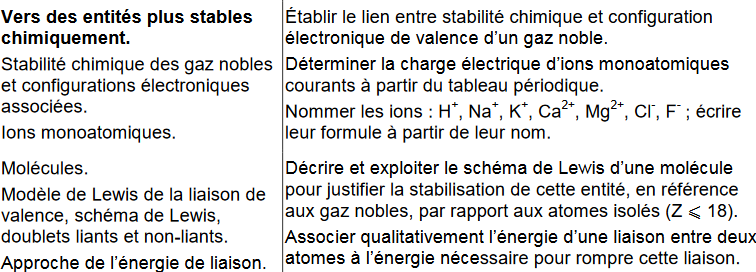
\includegraphics[width=1\textwidth]{Bo.png}
\end{center}
}


\doc{2}{Exercices dans le livre scolaire}{
		\begin{enumerate}
			\item Stabilité des entités chimiques : exercices 5, 6 et 10 page 115;
			\item La formation des ions : exercices 7 et 13 p115;
			\item Le modèle de Lewis : exercices 9, 15, 16 p 116.
		\end{enumerate}
}
	\noindent \textbf{Quiz sur la lumière et les spectres}
\begin{figure}[ht]
	% \centering
	\subfloat[Quiz 1 : Les entités stables : \hfill \url{https://forms.office.com/r/gyEtmKM673?origin=lprLink}]{
\includegraphics[width=.2\textwidth]{Quiz1.png}}\hfill
	\subfloat[Quiz 2 : Formation des ions : \hfill \url{https://forms.office.com/r/wTVu3Hmwup?origin=lprLink}]{
\includegraphics[width=.2\textwidth]{Quiz2.png}}\hfill
	\subfloat[Quiz 3 : Modèle de Lewis : \hfill \url{https://forms.office.com/r/S14tuwsY1V?origin=lprLink}]{
\includegraphics[width=.2\textwidth]{Quiz3.png}}\hfill
	\subfloat[Pour aller plus loin : \hfill \url{https://learningapps.org/view23412425}]{
\includegraphics[width=.2\textwidth]{PourAllerPLusLoin.png}}\hfill

\end{figure}

\clearpage
\section*{Introduction}

Il est rare de trouver dans la nature de la matière à l'état atomique : on a souvent affaire à des ions ou à des molécules. Dans ce chapitre, on cherche à comprendre la formation de ces composés, et même, à la prévoir à partir de la position des atomes dans le tableau périodique de \bsc{Mendeleïev}.

\begin{figure}[ht]
	\centering
	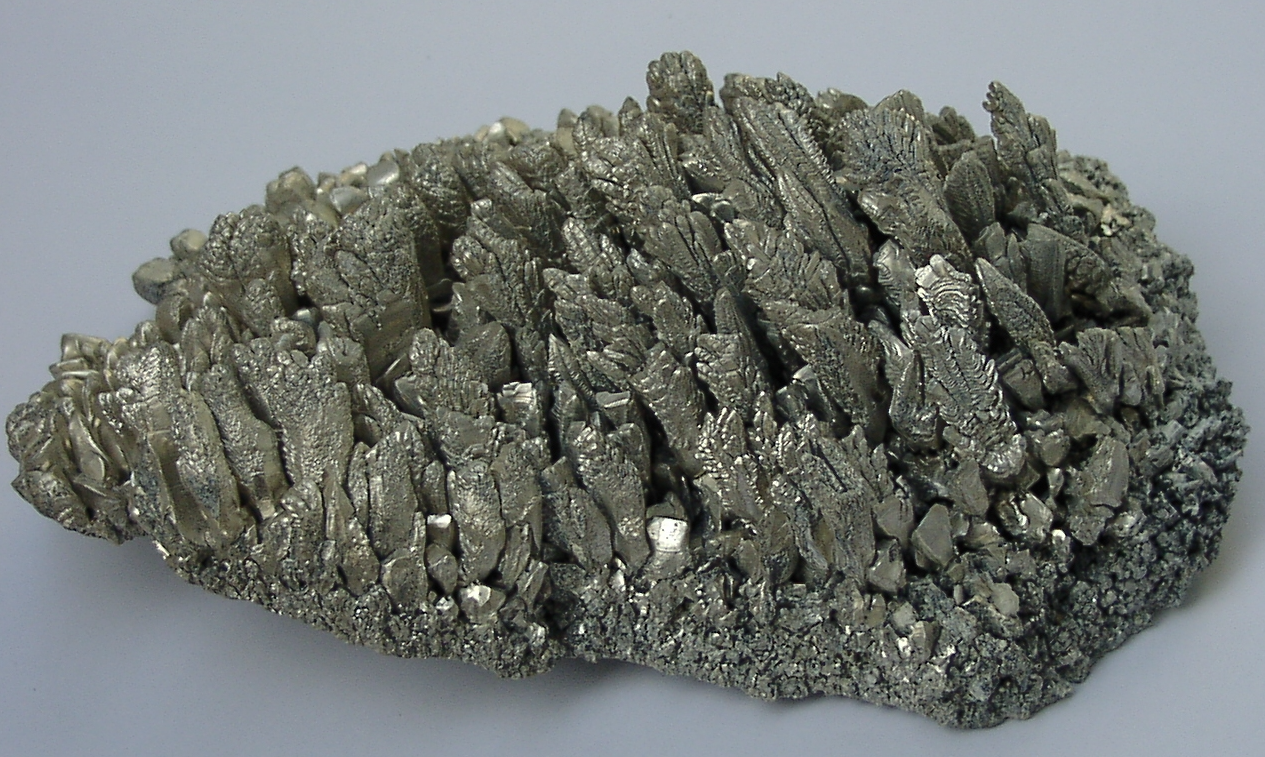
\includegraphics[width=.31\textwidth]{Magnesium.png}\hspace{2cm}
	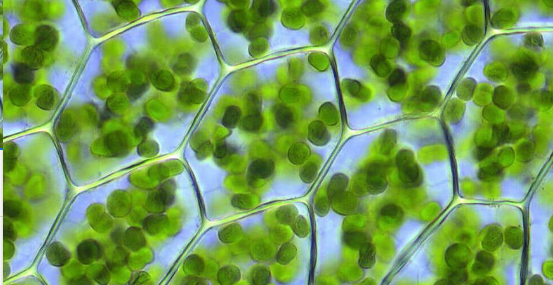
\includegraphics[width=.38\textwidth]{chlorophylle.png}
	\caption{Illustration de deux composés, l'un sous sa forme atomique le magnésium (à gauche) l'autre sous sa forme moléculaire la chlorophylle (à droite).}
\end{figure}
\vspace{-.5cm}
\section{Condition de stabilité d'une entité}

\begin{center}
	\textit{référence : Le livre scolaire page 111-112}
\end{center}

Dans cette première section, on s'intéresse aux conditions nécessaires à la stabilité d'une espèce chimique.

\begin{definition}{Définition 1 - Stabilité}

Une entité chimique est stable lorsqu'elle ne subit pas de désintégration. C'est à dire lorsqu'il y a un équilibre entre le nombre de neutrons et le nombre de protons.

\end{definition}

Lorsqu'un atome est petit, il contient pratiquement le même nombre de protons que de neutrons. Les entités stables plus volumineuses ont légèrement plus de neutrons que de protons. Les entités chimiques deviennent instable dès que l'écart entre le nombre de protons et de neutrons devient très important comme par exemple dans le cas de l'uranium \isotope{238}{92}{U}.


\subsection{Les gaz nobles}
\begin{minipage}{.8\textwidth}

La famille des gaz nobles (hélium, néon, etc) est l'ensemble des éléments\medskip

situés dans \textbf{\textcolor{blue}{la 18ème colonne}}  du tableau périodique. Ceux-ci jouissent d'une \textbf{stabilité exceptionnelle}.

\exo{1}{Configuration électronique des gaz nobles}{Écrire la configuration électronique des trois premiers gaz nobles (hélium, néon, argon).

\begin{itemize}
	\item He : $1s^2$
	\item Ne : $1s^22s^22p^6$
	\item Ar : $1s^22s^22p^63s^23p^6$
\end{itemize}
}
\end{minipage}\hspace{1cm}
\begin{minipage}{.2\textwidth}
	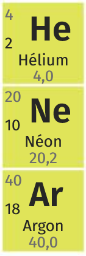
\includegraphics[scale=.8]{GazNobles.png}
\end{minipage}\bigskip

La configuration électronique de la couche de valence des gaz nobles est de la forme : 

\begin{itemize}
	\item $1s^2$ pour l'hélium He;
	\item  $ns^2np^6$ pour les autres gaz nobles. 
\end{itemize}\medskip

La couche de valence des gaz nobles est donc \textbf{\textcolor{blue}{complète}}.

\subsection{Des règles de stabilité}

L'étude des gaz nobles nous permet de dégager un lien entre configuration
électronique et stabilité. On énonce ainsi une règle générale de stabilité :

\begin{Proposition} {Règles de stabilité}
	\textbf{La règle de duet : } Les atomes dont le numéro atomique est proche de celui de l'hélium $Z=2$ ont tendance a adopter sa configuration à deux électrons $1s^2$.

	\textbf{La règle de l'octet : } Les autres atomes ont tendance à adopter la configuration électronique externe de l'atome dit gaz noble le plus proche avec huit électrons ($ns^2np^6$)
\end{Proposition}

\exo{2}{Atome d'oxygène}{
\begin{enumerate}
	\item En vous aidant de votre tableau périodique, trouver le numéro atomique de l'oxygène et écrire sa configuration électronique.\medskip
	
	Oxygène a un numéro atomique de 8, donc il possède 8 électrons\medskip

	$1s^22s^22p^4$

	\item Respecte-t-il la règle de stabilité des atomes ? \medskip
	
	Non Il ne respecte pas la règle du duet ni celle de l'octet. 
 \end{enumerate}
}
\section{En quête de stabilité}

Pour obtenir une configuration électronique stable, les atomes ont deux options, ils peuvent : 
\begin{itemize}
	\item\textbf{gagner ou perdre des électrons}, ils forment alors des \textbf{anions} ou des \textbf{cations} ;
	\item \textbf{partager leurs électrons} avec d'autres atomes, ils forment alors des \textbf{molécules}.
\end{itemize}

\subsection{Formation des ions}

Pour adopter la même configuration électronique que celle d'un gaz
noble, un atome peut gagner ou perdre des électrons. Il forme alors un \textbf{ion monoatomique} stable.

\exo{3}{Formations d'ions monoatomiques}{
\begin{enumerate}
	\item Quel ion l'oxygène étudié à l'\bsc{exercice 2} va-t-il tendre à former ?\medskip
	
	Il va former l'ion oxyde de formule $O^{2-}$ car il va chercher à gagner deux électrons pour compléter sa couche de valence

	\item Même question pour le magnésium \isotope{24}{12}{Mg}.  \textit{On pourra commencer par déterminer sa configuration électronique.}\medskip
	
	Mg : $1s^22s^22p^63s^2$

	Le Magnésium va chercher à perdre deux électrons pour satisfaire la règle de l'octet. Il va alors former l'ions $Mg^{2+}$.
\end{enumerate}
}

La charge que portera un ion dépend de la colonne du tableau périodique
dans laquelle l’atome correspondant se trouve.

\subsection{Formation des molécules}

En opérant un partage d'un ou de plusieurs électrons avec d'autres atomes, un atome peut devenir stable : c'est l'objet des \textbf{molécules}.

\subsubsection{Liaison covalente et doublets non-liants}

\begin{definition}{Définition 2 - Liaison covalente}
	La \textbf{liaison covalente} est une mise en commun de deux électrons de valence entre deux atomes.
\end{definition}


On représente une liaison covalente par un tiret entre les deux atomes concernés:
\begin{center}
\chemfig[atom sep =2em]{A-B}\hspace{3cm} \chemfig{A=B}\hspace{3cm} \chemfig{A~B}
\end{center}
Une liaison covalente peut être simple, double ou même triple ! 


\begin{definition}{Définition 3 - Doublet non-liant}
	\medskip 

	Les électrons de valence qui ne participent pas aux liaisons covalentes sont répartis en doublets d'électrons appelés doublets non-liants. 
\end{definition}

Chaque \textbf{doublet non liant} est représentaé par un tiret placé sur l'atome considéré. Comme l'exemple ci-dessous le doublet non-liant est dessiné sur l'atome B.
\begin{center}
	\chemfig[atom sep =2em]{A-\charge{90=\|}{B}}
\end{center}

Chaque atome respectera donc soit la règle du duet, soit la règle de l'octet. Les formules de Lewis des molécules permettent de vérifier le respect de ces règles en comptabilisant les électrons des liaisons covalentes et des doublets non liants pour chaque atome de la molécule.




\subsubsection{Formule de Lewis}

La formule brute d'une molécule comporte des carences d'informations : elle
ne renseigne pas sur l’agencement des atomes ou sur la disposition des doublets
électroniques. La représentation de Lewis permet de pallier ces problèmes. Elle
permet également de vérifier facilement le respect de la règle de stabilité.

\begin{definition}{Définition 4 - Formule de Lewis}

C'est une représentation en deux dimensions de la structure électronique externe des atomes composant une molécule

\end{definition}

% \begin{Exercice}{Exercice : Déterminer la formule de Lewis de l'eau $H_2O$}
\exo{4}{Représentation de Lewis de la molécule d'eau}{
	\begin{minipage}{.65\textwidth}
		\begin{enumerate}
		\item Donner la configuration électronique de l'oxygène O et de l'hydrogène H.\medskip
		
		% \dotfill \medskip

		% \dotfill

		H : $1s^1$ et O : $1s^22s^22p^4$

		\item Combien d'électrons de valence sont mis en jeu ? \medskip
		
		% \dotfill \medskip

		% \dotfill

		Hydrogène possège 1 électron de valence. L'oxygène en possède 2. 

		\item Représenter la formule de Lewis de l'eau.
	\end{enumerate}
		\end{minipage}
		\begin{minipage}{.35\textwidth}
		\begin{center}
			\begin{tikzpicture}
				\draw[step = 0.5, color = black!30] (-.5,-1) grid++ (3.5,3);
				\chemfig{H-[:30]\charge{45=\|,135=\|}{O}-[:-30]H}\par \setchemfig{atomsep=2.5em}
			\end{tikzpicture}
		\end{center}
	\end{minipage}
}
\clearpage

\subsubsection{Énergie de liaison}

De manière générale, il faut \textbf{fournir} de l’énergie pour briser une
liaison. À l’inverse, lorsqu’une liaison chimique entre deux atomes est créée,
cela \textbf{libère} de l’énergie.




\begin{minipage}{.6\textwidth}
% \begin{figure}[ht]
	\centering
	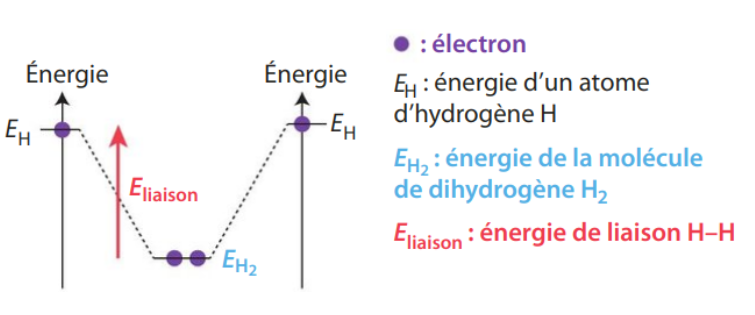
\includegraphics[width=1\textwidth]{SchemaEnergieLiaison.png}
% \end{figure}
	% \begin{tikzpicture}
% 	\draw[ultra thick, -latex] (-1,0) -- (-1,2.3);
% 	\draw[ultra thick, -latex]	(1+.5,0) -- (1+.5,2.3);
% 	\draw[dashed] (-1,1.8) -- (-.2,0.1)--(0.2+.5,.1)--(1+.5,1.8);
% 	\draw[blue] (0.2+.5,.1) node{$\bullet$};
% 	\draw[blue] (-.2,.1) node{$\bullet$};
% 	\draw[blue] (-1,1.8) node{$\bullet$};
% 	\draw[blue] (1+.5,1.8) node{$\bullet$};
% 	\draw (-1.5,1.8) node{$E_{\rm H}$};
% 	\draw (1.5+.5,1.8) node{$E_{\rm H}$};
% 	\draw[ultra thick, -latex, red] (-.7,0)--(-.7,1.6) node[midway, right]{$E_{\rm liaison}$};
	

	
% \end{tikzpicture}
\end{minipage}
\begin{minipage}{.5\textwidth}
\begin{tabular}{|c|c|}
	\hline 
	Liaison & Énergie ($\rm J\cdot mol^{-1}$)\\ \hline
	\chemfig[atom sep =2em]{C-H} & 413 \\ \hline
	\chemfig[atom sep =2em]{C-C} & 248 \\ \hline
	\chemfig[atom sep =2em]{O-H} & 463 \\ \hline
	\chemfig[atom sep =2em]{O=O} & 496 \\  \hline
\end{tabular}
\end{minipage}

\begin{definition}{Définition - Énergie de liaison}

	L'\textbf{énergie de liaison} est l'énergie requise pour rompre toutes les liaisons covalentes d'une mole de la molécule considérée\medskip

	Elle se mesure en $\rm J\cdot mol^{-1}$
	\end{definition}

\exo{6}{Molécule d'eau (énergie de liaison)}{

\begin{itemize}
	\item En vous aidant de sa représentation de \bsc{Lewis}, établir la liste des liaisons covalentes que comporte une molécule d'eau.\medskip
	
	% \dotfill \medskip

	% \dotfill
	
	Il y a deux liaisons covalente (O-H) dans la molécule d'eau.

	\item Quelle est l'énergie de liaisons d'une seule de ces liaisons covalentes ?\medskip
	
	% \dotfill \medskip

	% 	\dotfill

	Chaque liaison Oh a une énergie de liaison de 463 SI. 

	\item Calculer l'énergie de l'ensemble des liaisons de la molécule d'eau.\medskip
	
	L'énergie totale est de $E_h = 926 ~\rm J\cdot mol^{-1}$.
\end{itemize}
}
\end{document}

%%
%% FIN DU DOCUMENT
%%
